\chapter{Evaluation}\label{chap:evaluation}
Through the use of the framework described in the previous chapter, we evaluate four different algorithms for next-activity prediction side-by-side: Two implementations that mimic Evermann et al. and Schönig et al, and the PFS and SP2 approaches presented in \autoref{chap:taking-inspiration}. For each model, we will analyze the four different approaches for structuring the training data for performance differences from \autoref{chap:training-framework}.

First we justify our choice of datasets in \autoref{sec:dataset-choice}. As we follow the KDD process, we then lead through the data preprocessing and transformation phases in \autoref{sec:eval:data-preprocessing} and \autoref{sec:eval:data-transformation}. The latter section also covers the strategy used to engineer the SP-2 and PFS features. Then, the test setup and the used training strategy is presented in \autoref{sec:eval:test-setup}, followed by the set of criteria by which we judge the results in \autoref{sec:eval:criteria}. Finally, the chapter ends with the presentation in \autoref{sec:eval:results} and discussion of the results in \autoref{sec:eval:discussion}. Used and relevant technologies are highlighted in each sections.

\section{Choice of dataset}
\label{sec:dataset-choice}
In \autoref{sec:intro:contribution}, we criticized the great variety of datasets used to evaluate approaches in Predictive Process Monitoring. While we can not establish a standard, we ensure comparability of our results to a variety of works by evaluating the four models on eight datasets in total, coming from the following sources:

\begin{itemize}
    \item BPIC11, an event log from cases in a Gynaecology department a Dutch Academic Hospital~\cite{BPIC2011}
    \item BPIC12, an event log for loan and overdraft applications from a Dutch Financial Institute~\cite{BPIC2012}
    \item BPIC15 provides logs by five Dutch municipalities. It contains all building permit applications over a period of approximately four years. It is divided into one dataset per municipality, referred to as BPIC15-1 to BPIC15-5 in the following~\cite{BPIC2015}
    \item Helpdesk Log, TODO TODO TODO
\end{itemize}
\todo[inline]{Check out the helpdesk log and see if it's worth it...}

We picked the three BPIC datasets as we believe that they cover a spectrum of process complexity. The least complex end of it is marked by BPIC12, which covers a loan application process from a financial institution with a small variance in trace length and a very small number of different activities. The complex end is marked by BPIC11, which covers patient treatments in a hospital. This results in logs of longer traces and an especially high number of distinct activities. BPIC15 resides relatively in the middle of the two, as \autoref{tab:dataset-characteristics} indicates.

While process models were easily mined for BPIC12\footnote{Citation needed}, they were more complex for BPIC15~\cite{van2015benchmarking}, and barely obtained for BPIC11. Furthermore we take the increasing number of distinct activities to be a measure of complexity.

Furthermore, these datasets allow us to compare our findings to the following works, which also worked on next-element predictions. When comparing, it is important to differentiate between the works that focused on case-specific predictions like us and those that focused on whole event streams:

\begin{itemize}
    \item Predicting the next element in a stream, not specific to a case
    \begin{itemize}
        \item BPI12: Tax et al.~\cite{tax2018interdisciplinary, tax2017}
        \item BPI12: Evermann et al.~\cite{evermann2016}
    \end{itemize}
    \item Predicting the next element for a specific case
    \begin{itemize}
        \item BPI12: Böhmer et al.~\cite{boehmer2018probability}
    \end{itemize}
\end{itemize}

\begin{table}[]
\centering
\begin{tabular}{lrrrrrrr}
\textbf{Dataset} & \textbf{min TL} & \textbf{max TL} &  \textbf{mean TL} & \textbf{\# Traces} & \textbf{\# Events} & \textbf{\# Activities} \\
\hline
\textbf{BPIC11} & 1 & 1 814 & 131.49 & 1 143 & 150 291 & 524\\
\textbf{BPIC12} & 3 & 96 & 12.56 & 13 087 & 164 506 & 23\\
\textbf{BPIC15-1} & 2 & 101 & 43.55 & 1199 & 52 217 & 398\\
\textbf{BPIC15-2} & 1 & 132 & 53.31 & 832 & 44 354 & 410\\
\textbf{BPIC15-3} & 3 & 124 & 42.35 & 1409 & 59 681 & 383\\
\textbf{BPIC15-4} & 1 & 116 & 44.91 & 1053 & 47 293 & 356\\
\textbf{BPIC15-5} & 6 & 154 & 51.10 & 1156 & 59 083 & 389\\
\end{tabular}
\caption{Properties of the traces contained in the used datasets. TL abbreviates trace length.}
\label{tab:dataset-characteristics}
\end{table}

\section{Data preprocessing}
\label{sec:eval:data-preprocessing}
In the first step of the KDD process~\cite{fayyad1996data}, the data is preprocessed to eliminate generally known properties that hinder machine learning model performance. In our case, this encompassed three steps for all datasets:

\begin{enumerate}
    \item Drop all columns which exhibit zero entropy, i.e. which contain only a single value
    \item Eliminate features which correlate strongly. To account for categorical correlation, the bias-corrected version of Cramér's~V~\cite{bergsma2013bias} is used.
\end{enumerate}

In step 1, one column was dropped in BPIC11 and two were dropped in BPIC17.
In step 2, the bi-directional results in \autoref{fig:BPIC11-correlation-heatmap} from Cramér's V revealed that the variables \texttt{Producer code}, \texttt{Activity code} and \texttt{Specialism code} correlate strongly with many others in the BPIC11 dataset. Thus, these were dropped. As evidenced in \autoref{fig:BPIC12-correlation-heatmap}, the BPIC12 dataset with its small number of features did not require any removals. In the BPIC17 dataset, \texttt{EventID} and \texttt{OfferID} were removed for being identifiers, and \texttt{Action} for its perfect correlation with \texttt{concept:name}. The correlation measurements are on display in gdskjl
\todo[inline]{create table with features, and indicate which ones were removed}

The activities described above were conducted in JupyterLab notebooks~\cite{web:jupyter}, where Anaconda~\cite{web:anaconda} was used to create a stable development environment. The OpyenXes~\cite{web:opyenxes} library proved to be especially useful for parsing the raw XES logs from BPIC.

\section{Data transformation}
\label{sec:eval:data-transformation}
Having removed unneeded features, the remaining ones were encoded following standard practice. Each numerical feature $x$ was normalized with values specific to each trace using the min-max method:

$$normalize(x) =
\begin{cases}
\frac{x-min(x)}{max(x)-min(x)} & \text{if } min(x) \neq max(x)\\
1 & \text{otherwise}
\end{cases}
$$

Categorical features without ordinal properties, which were all of them, were encoded using one-hot encoding if possible. In the case of the input for Evermanns model, the concatenation of activity name and resource ID was encoded with dictionary encoding, as demonstrated in his paper~\cite{evermann2016}.

\subsection*{SP-2 feature engineering}
For every trace, SP-2 features mark whether an activity has occured yet. Thus, these features are engineered in an iterative fashion, as \autoref{lst:sp2-generation} outlines. For every trace, a new data frame \texttt{sp2\_df} is created and the occurence of the first activity is marked inside it. Now, a loop begins over the remaining steps, where each previous row inside \texttt{sp2\_df} is copied into the currently indexed row and the presence of the current activity is marked. This repeats itself until the trace has been processed completely.

\begin{listing}[ht]
\begin{minted}{python}
# Dataframe initialization with zeroes
sp2_df = pd.DataFrame(columns=activity_labels,
                      index=range(0,len(t)),
                      dtype=np.bool)
for col in sp2_df.columns: sp2_df[col].values[:] = 0

# mark first occuring SP-2 
cname = "{0}{1}".format(sp2_prefix, t[target_col][0])
sp2_df[cname].values[0]  = 1

# copy over values from last row and
# set activity labels accordingly
for i in range(1,len(t)):
    first_activity_name = t["concept:name"].iloc[i]
    col = "{0}{1}".format(sp2_prefix,first_activity_name)
    
    sp2_df.values[i] = sp2_df.values[i-1]
    sp2_df[col].values[i] = 1
\end{minted}
\caption{Generating SP-2 features for a single trace \texttt{t} and a specific target column \texttt{target\_col}.}
\label{lst:sp2-generation}
\end{listing}

\subsection*{Sub-sequence feature engineering}
The sub-sequence features for the PFS model were created with the help of the \textit{prefixspan-py} library~\cite{web:prefixspan-py}. As \autoref{lst:pfs-mining} shows, the library greatly facilitates obtaining closed sub-sequences ranked by support, returning a two-dimensional array of sub-sequences, with one array per sub-sequence. The sequences are mined from the entirety of traces.

\begin{listing}[ht]
\begin{minted}{python}
prefixspan_traces = PrefixSpan(encoded_traces)
closed_sequences = prefixspan_traces.topk(25, closed=True)
\end{minted}
\caption{Obtaining closed sequences using the \textit{prefixspan-py} library.}
\label{lst:pfs-mining}
\end{listing}

After mining the sequences, a loop is executed for every trace, shown in \autoref{lst:subsequence-feature-creation}. For each index \verb=i= it is checked whether any of the mined subsequences starts at that position. This is checked by peeking ahead of \verb=i= for the length of the subsequence. As in the case of the SP-2 features, the occurence of a subsequence is marked with a boolean flag from the row that it occured in onwards.

\begin{listing}[ht]
\begin{minted}{python}
subseq_df = pd.DataFrame(columns=subseq_labels,
                         index=range(0,len(t)),
                         dtype=np.bool)
subseq_df[:].values[:] = False
activity_codes = t[target_col].map(event_to_int)
tlen = len(t)

for i in range(0, tlen):
  # loop through all subsequences
  for subseq_idx, subseq in enumerate(ps):
    if tlen <= i+len(subseq): continue
            
    # check if subseq takes place in the following steps
    subsequence_found = True
    j = 0
    
    while subsequence_found and j < len(subseq):
      if subseq[j] != activity_codes[j+i]:
        subsequence_found = False
        j += 1

    # if subseq took place, subsequence_found is still true
    if subsequence_found:
      subseq_df.values[j+i:,subseq_idx] = True
\end{minted}
\caption{Enriching a trace \texttt{t} with sub-sequence features by detecting those that are contained inside it.}
\label{lst:subsequence-feature-creation}
\end{listing}

\subsection*{Target construction}
For each itemset $i_t$ at a given timestep $t$, the prediction target $a_t$ was constructed. While the itemset could also contain data attributes, the prediction target solely consisted of the activity name. For the target of the last $t$ of a trace, a marker for denoting the end of the sequence, \verb=EOS=, was introduced.
As the goal is to predict the next activity, the column containing this information needed to be identified in the data. For all three datasets, this turned out to be \verb=concept:name=.

\section{Test setup}
\label{sec:eval:test-setup}
To conduct the experiments, Docker containers were built with the development Anaconda environment inside them~\cite{web:docker}. Using a version of Docker for GPU applications running on NVIDIA hardware~\cite{web:nvidia-docker}, each network-batch-formatting combination was trained and evaluated on a single NVIDIA K80 GPU of the HPI FutureSOC Lab~\cite{web:fsoc}. The complete source code used for evaluation is publicly available on GitHub at \href{https://github.com/flxw/master-thesis-code}{flxw/master-thesis-code}.\\

All datasets were split into training and test sets of complete traces. While $25\%$ of the traces were used for validation and testing, the remaining $75\%$ were used for training purposes. The sets were shuffled and stratified to contain an approximately similar distribution of trace lengths.

Each model implementation was trained successively with each data formatting variant on a single GPU. A model was saved when its validation loss, calculated on the test set, hit a new record low. If the validation loss did not improve for 10 epochs, the training was interrupted. This is commonly referred to as early stopping. \autoref{tab:training-setup} illustrates information about the training setup of the networks side-by-side. As Evermann et al. made use of a version of Tensorflow that is deprecated as of the time of writing, our implementation in Keras can only be understood as an approximation. Evermann's implementation of an "unrolled LSTM" can only be approximated in Keras.

\begin{table}[ht!]
    \centering
    \begin{tabular}{lcccc}
        \textbf{Network}   & \textbf{Evermann} & \textbf{Schönig} & \textbf{SP2} & \textbf{PFS}\\
        \hline
        \textbf{Optimizer} & SGD\footnote{SGD stands for Stochastic Gradient Descent. Additionally setting the learning rate decay to $0.75$ at the $25^{th}$ epoch.} & \multicolumn{3}{c}{RMSprop} \\
        \textbf{Loss}      &\multicolumn{4}{c}{Categorical crossentropy}\\
        \textbf{Weight initializer} & Zeros & None & \multicolumn{2}{c}{Glorot normal}\\
        \textbf{Epochs}    & 50 & 100 & 150 & 150\\
        \textbf{Features}  & \makecell{Activity +\\Resource} & \multicolumn{3}{c}{All usable data attributes}\\
    \end{tabular}
    \caption{Used hyper-parameters for each model, with the number of epochs to be understood as the maximum number of epochs, as training may stop early}
    \label{tab:training-setup}
\end{table}

\section{Evaluation criteria}
\label{sec:eval:criteria}
The following three metrics are the focus in the evaluation of the sixteen model-formatting combinations:

\begin{enumerate}
    \item\textbf{Accuracy} - The share of correct next-activity predictions.
    \item\textbf{Resource consumption} - The amount of time and memory required during training.
    \item\textbf{Stability} - Whether the prediction accuracy changes as the trace progresses.
\end{enumerate}

While the first two criteria target the general usability of each model, the last one permits making a judgment about the stability of the predictions. It is inspired by the works of Francescomarino et al.~\cite{francescomarino2015} and Klinkmüller et al.~\cite{klinkmuller2018reliablemonitoring}. This allows better insights into how prediction accuracy develops over time, and facilitates building trust in the model, as indicated in the introduction of the thesis.

\section{Results}\label{sec:eval:results}
The three aforementioned criteria were applied to each model-batching combination on each dataset, and the results are presented in this section. By evaluation criterion, we go through the measurements. Most of the corresponding figures can be found in the Appendix, due to space reasons. \autoref{tab:network-info} lists dimensions which can have an impact on performance and will be referred to throughout the following subsections.

\begin{table}[htb!]
\centering
\begin{tabular}{lcccc}
\textbf{Dataset} & \textbf{Evermann et al.} & \textbf{Schönig et al.} & \textbf{SP2} & \textbf{PFS}\\
\hline
\hline
\textbf{BPIC11} & 1 & \makecell{n=655\\m=625} & \makecell{n=655\\m=625} & \makecell{n=655\\m=625\\ l=25} \\
\hline
\textbf{BPIC12} & 1 & \makecell{n=655\\m=625} & \makecell{n=655\\m=625} & \makecell{n=655\\m=625\\ l=25} \\
\hline
\textbf{BPIC17} & 1 & \makecell{n=655\\m=625} & \makecell{n=655\\m=625} & \makecell{n=655\\m=625\\ l=25} \\
\end{tabular}
\caption{Input and output vector dimensionalities for each dataset}
\label{tab:network-info}
\end{table}

\subsection*{Accuracy}
The overall accuracy is a good indicator of the prediction performance of a sequence-prediction model. In this section we will go over the model performances per batching strategy and explain the results. In \autoref{fig:max-accuracies-bpic2011} to \autoref{fig:max-accuracies-bpic2015-5}, the model performances per dataset are presented, grouped by batching strategy. The plots make apparent that only three models perform well consistently and that all react very differently to each batching strategy.

Looking at the performance of the EVM model across all datasets, it is evident that it is consistently outperformed. Its performance on the BPIC12 datasets represents an exception. We trace this lack of performance back to the application of an Embedding layer, which we suspect to require more data than included in most datasets to improve its internal data representation. The performance jump on the BPIC12 dataset corresponds nicely to the small number of activities and large number of traces in \autoref{tab:dataset-characteristics}, which helps the Embedding learn better.

Unsurprisingly, the individual batching strategy often results in slightly worse accuracies than the grouped batching strategy, with the exception of the BPIC12 dataset. We trace this back to the frequent adjustment of weights that might lead the loss optimization into local minima. In the trace length distributions in \autoref{appendix:trace-length-distributions}, the explanation for the high accuracy on BPIC12 with the individual batching strategy can be found. As this dataset has the highest number of traces and a relatively even distribution of lengths, the batches become too large, leading to lost optimization opportunities. With this knowledge, the strategy should be enhanced to split batches if they exceed a certain size threshold.

The padded strategy leads to consistently good results throughout the datasets and only loses accuracy on the BPIC11 datasets where the training set had to be shrunk because traces exceeded the length threshold.

While the batching strategies that provide the whole history to the model consistently see the SCH, SP2 and PFS models on par with at most $0.1$ difference, the windowed batching strategy leads to very different results depending on the dataset and the model. With the window size set to three, the model does not have many timesteps to learn from in any given sample. However, this loss of information does not impact the SP2 model. We assume that its SP-2 features encode the history that is cut away and thus help it come close to the general maximum accuracy of the dataset with the exception of BPIC11.

\begin{figure}
    \centering
    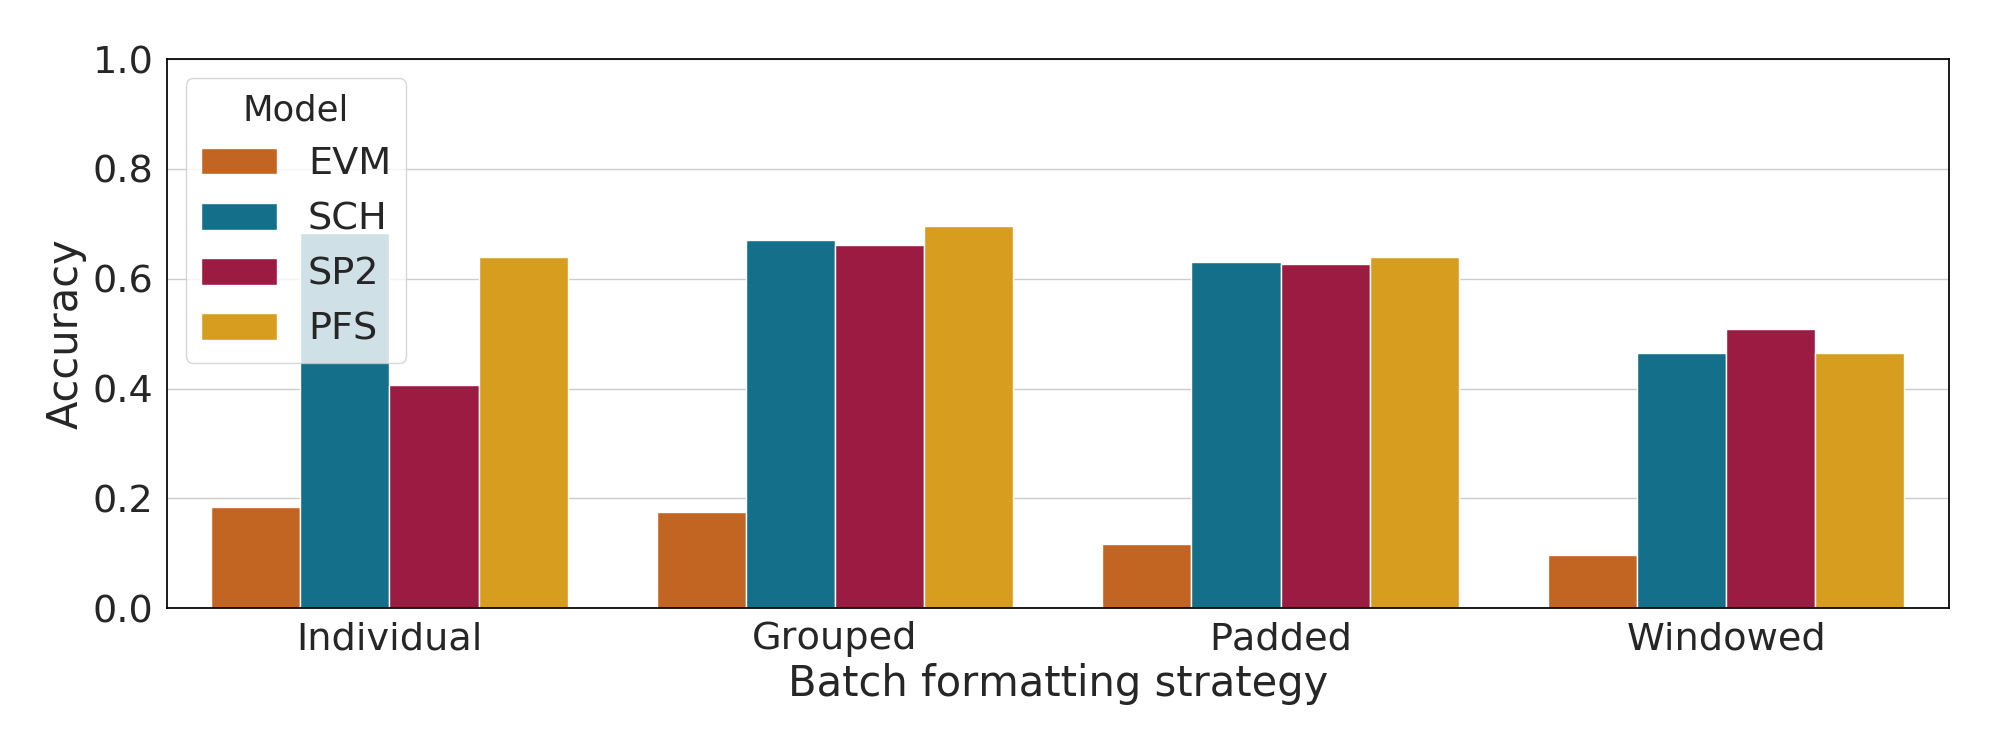
\includegraphics[width=\textwidth]{gfx/bpic2011/accuracies.png}
    \caption{Best accuracies obtained on the validation set on the BPI11 data}
    \label{fig:max-accuracies-bpic2011}
\end{figure}
\begin{figure}
    \centering
    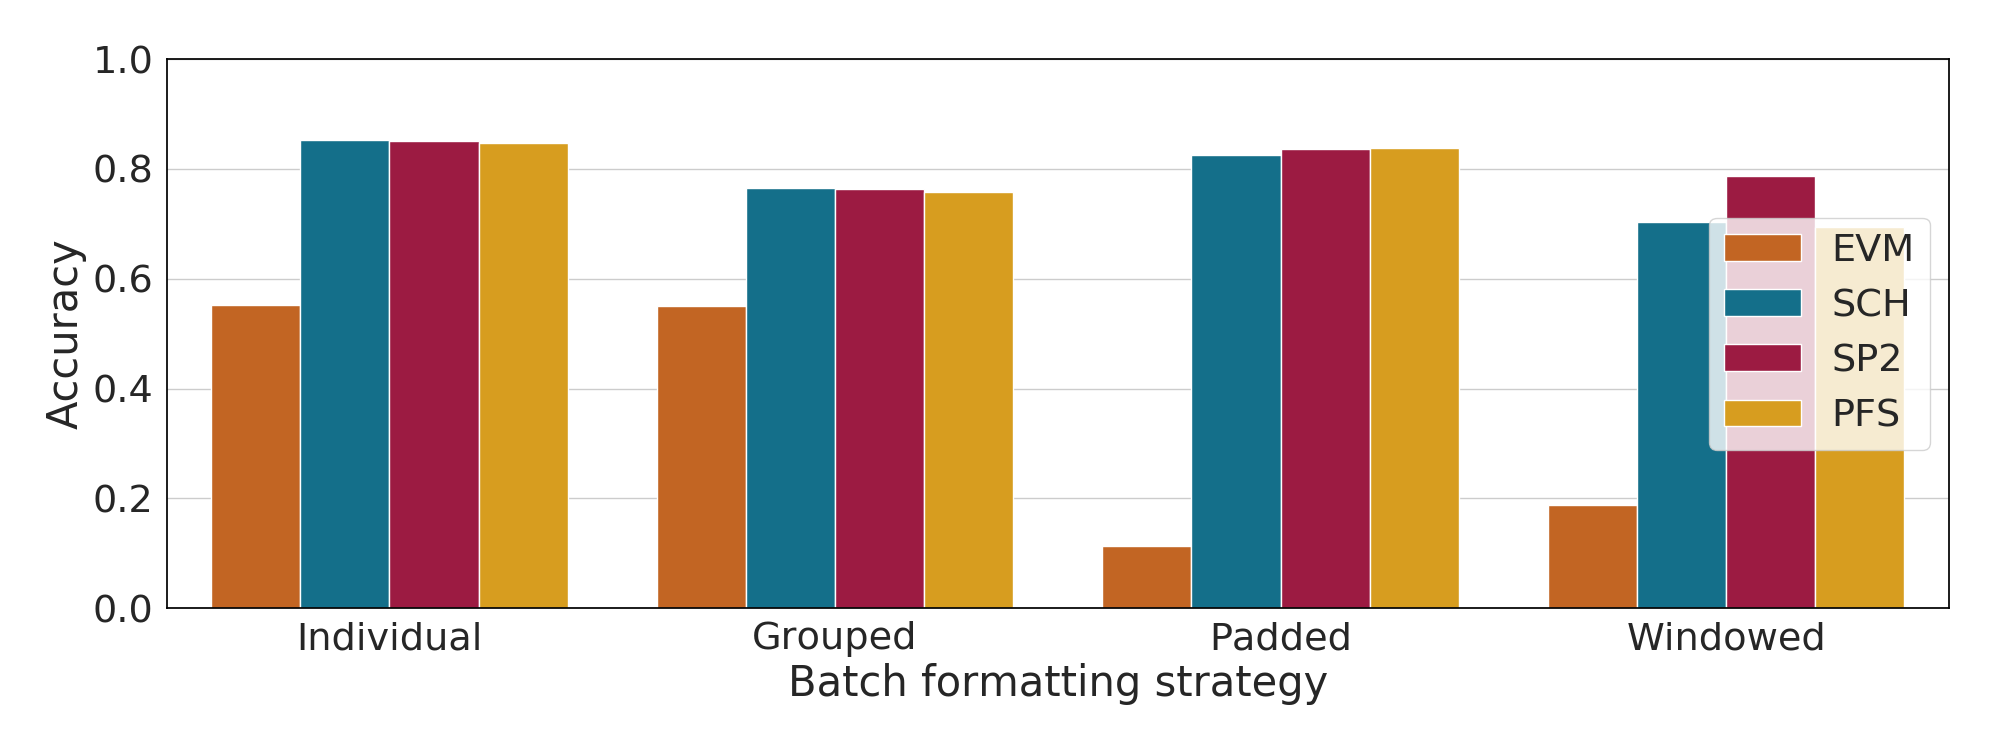
\includegraphics[width=\textwidth]{gfx/bpic2012/accuracies.png}
    \caption{Best accuracies obtained on the validation set on the BPI12 data}
    \label{fig:max-accuracies-bpic2012}
\end{figure}
\begin{figure}
    \centering
    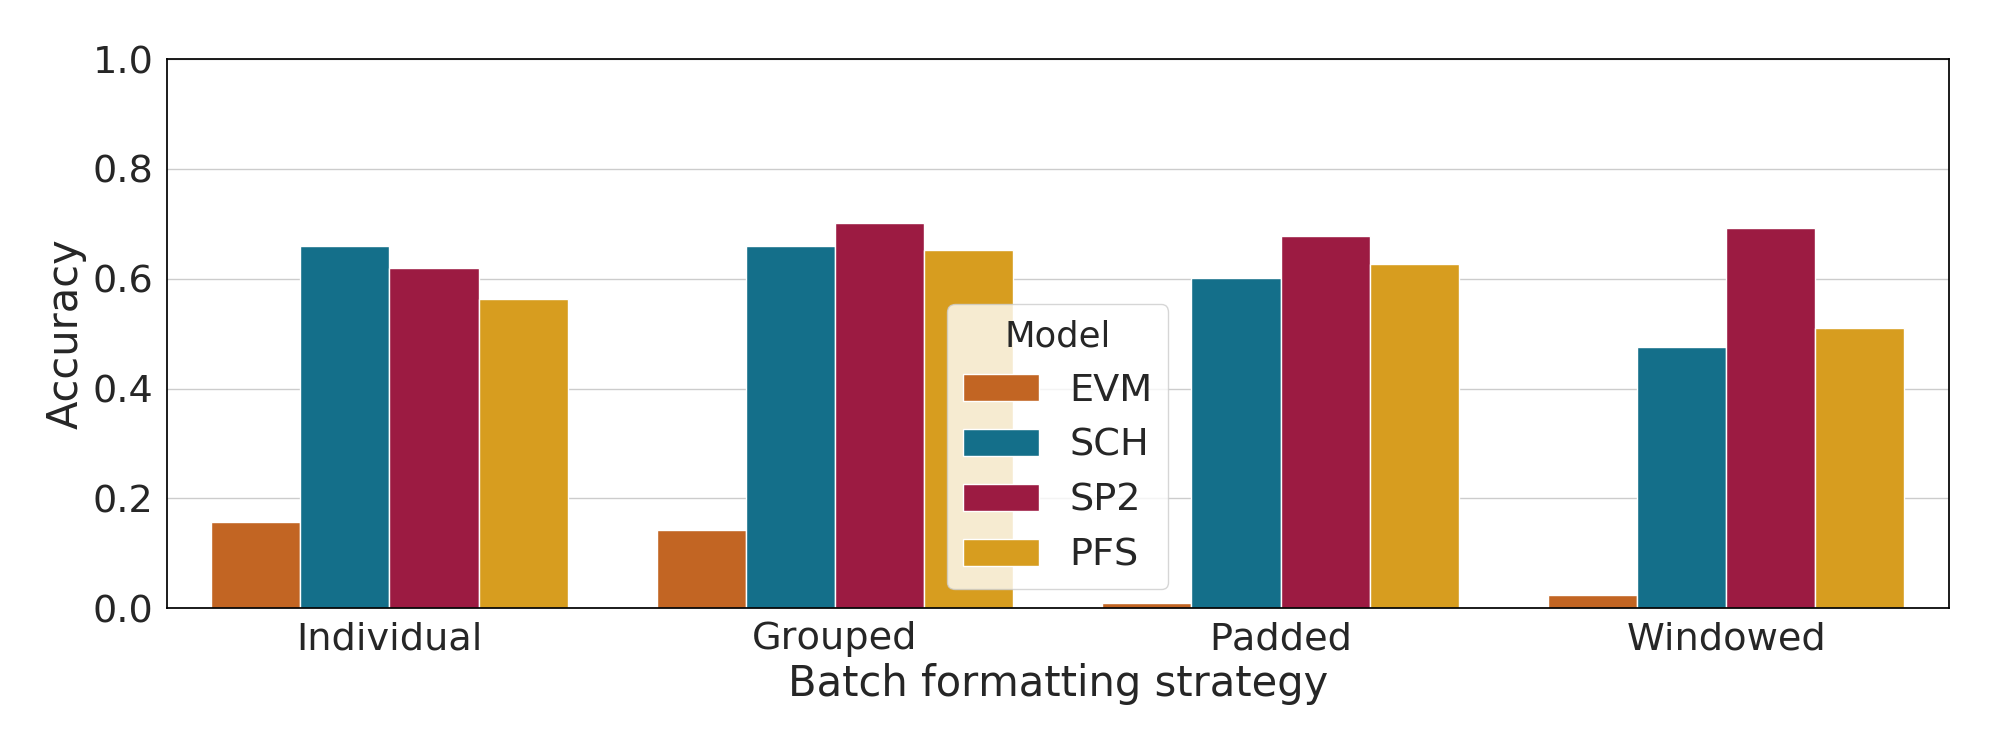
\includegraphics[width=\textwidth]{gfx/bpic2015_1/accuracies.png}
    \caption{Best accuracies obtained on the validation set on the BPI15-1 data}
    \label{fig:max-accuracies-bpic2015-1}
\end{figure}
\begin{figure}
    \centering
    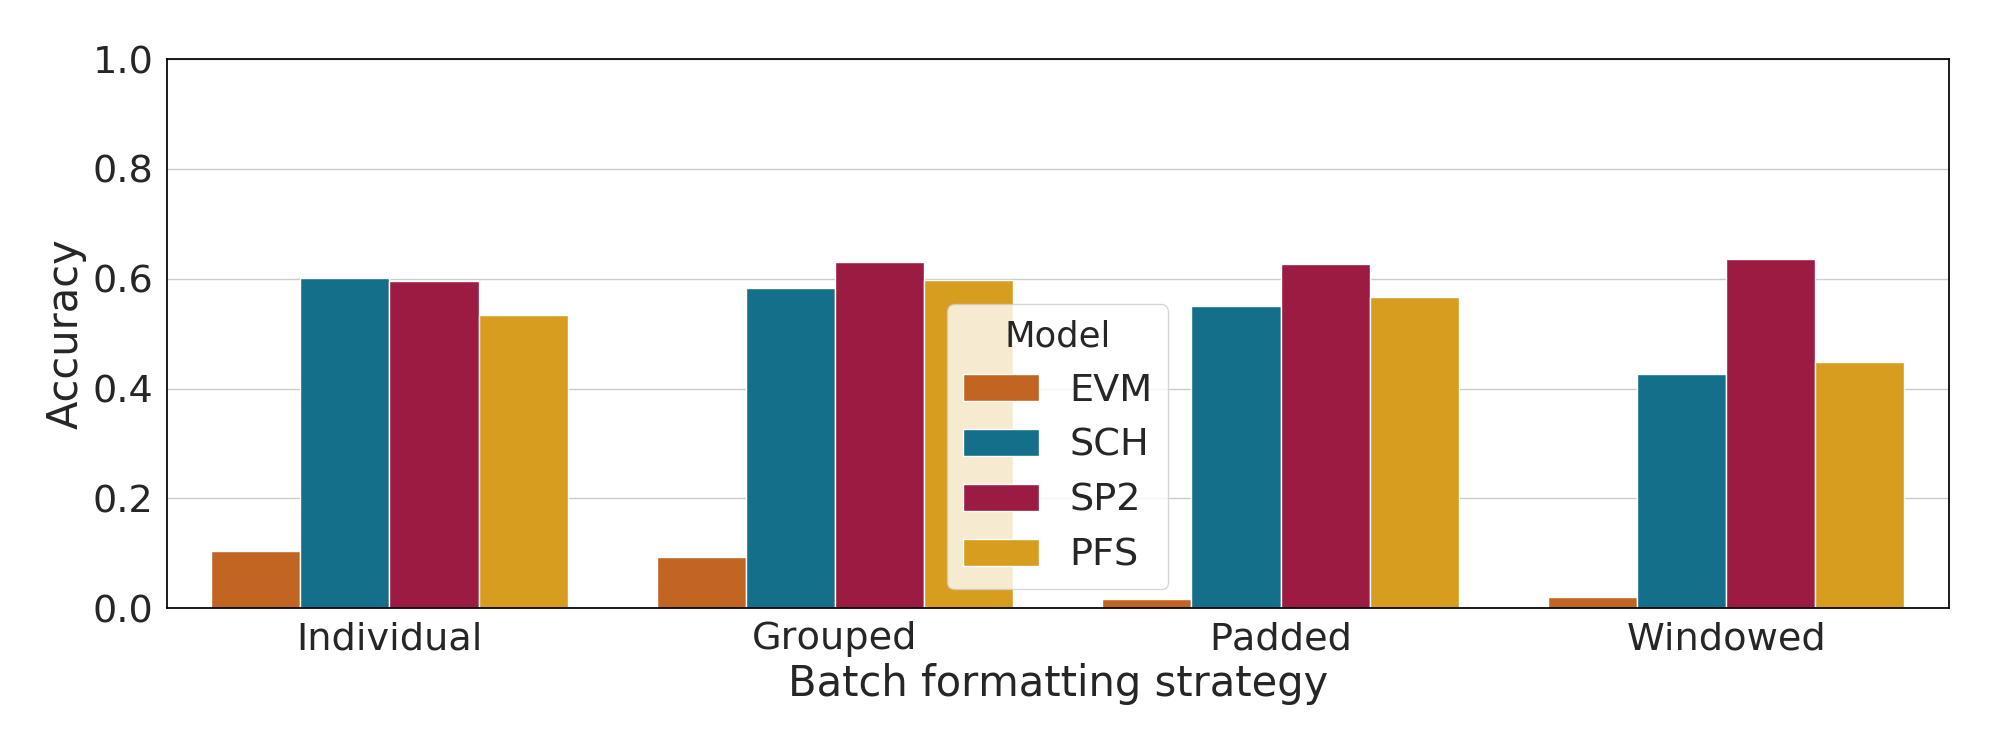
\includegraphics[width=\textwidth]{gfx/bpic2015_2/accuracies.png}
    \caption{Best accuracies obtained on the validation set on the BPI15-2 data}
    \label{fig:max-accuracies-bpic2015-2}
\end{figure}
\begin{figure}
    \centering
    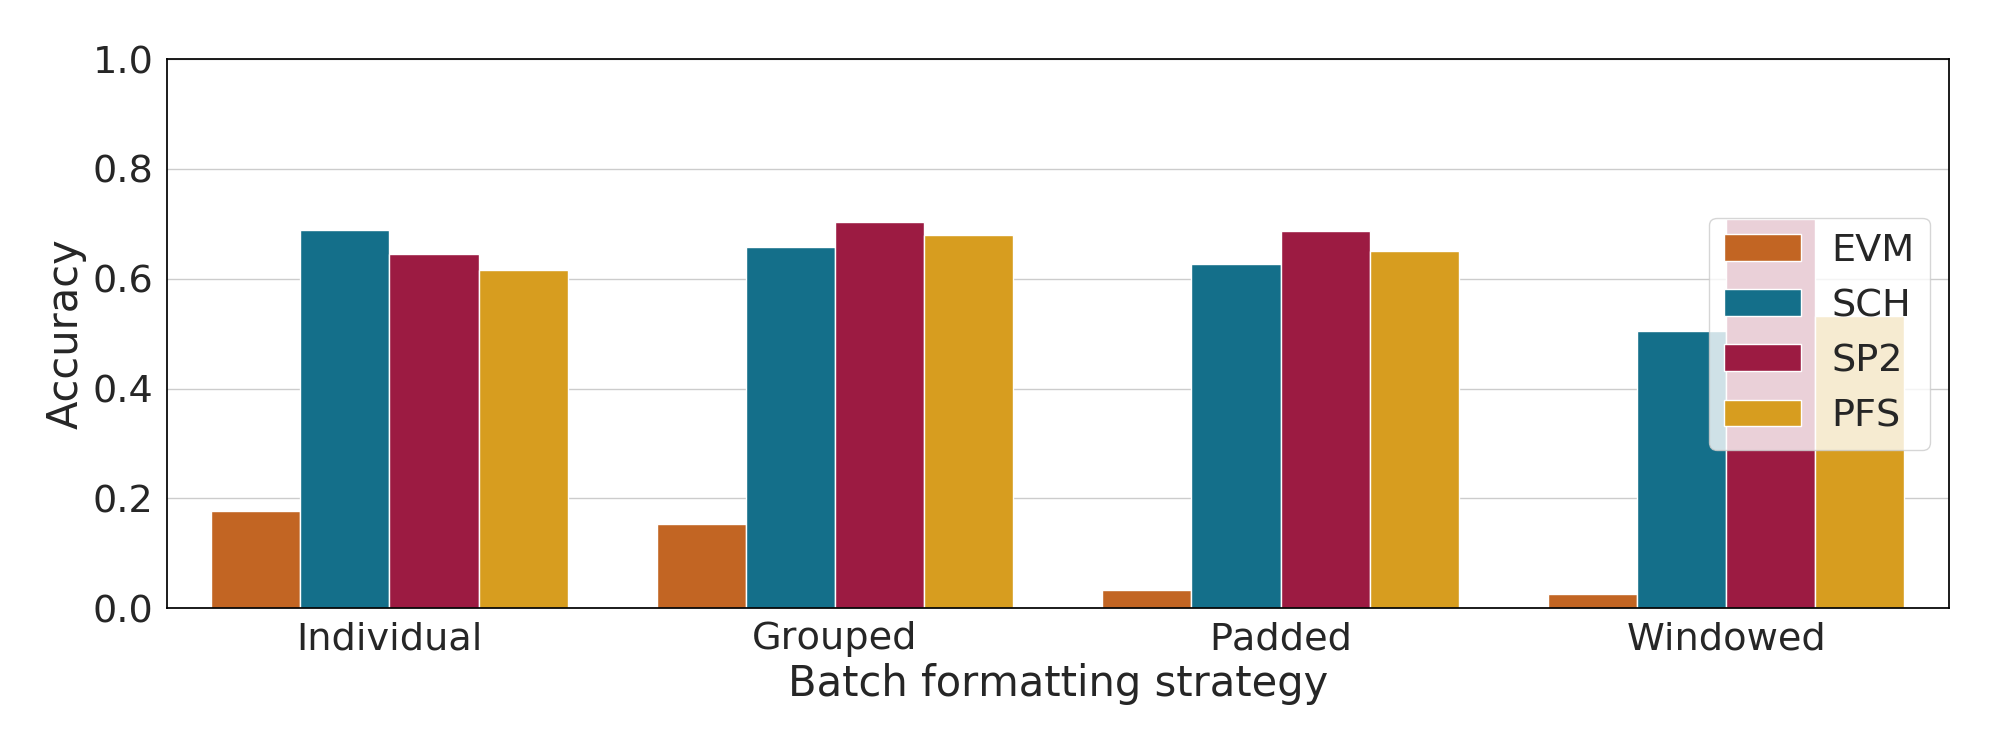
\includegraphics[width=\textwidth]{gfx/bpic2015_3/accuracies.png}
    \caption{Best accuracies obtained on the validation set on the BPI15-3 data}
    \label{fig:max-accuracies-bpic2015-3}
\end{figure}
\begin{figure}
    \centering
    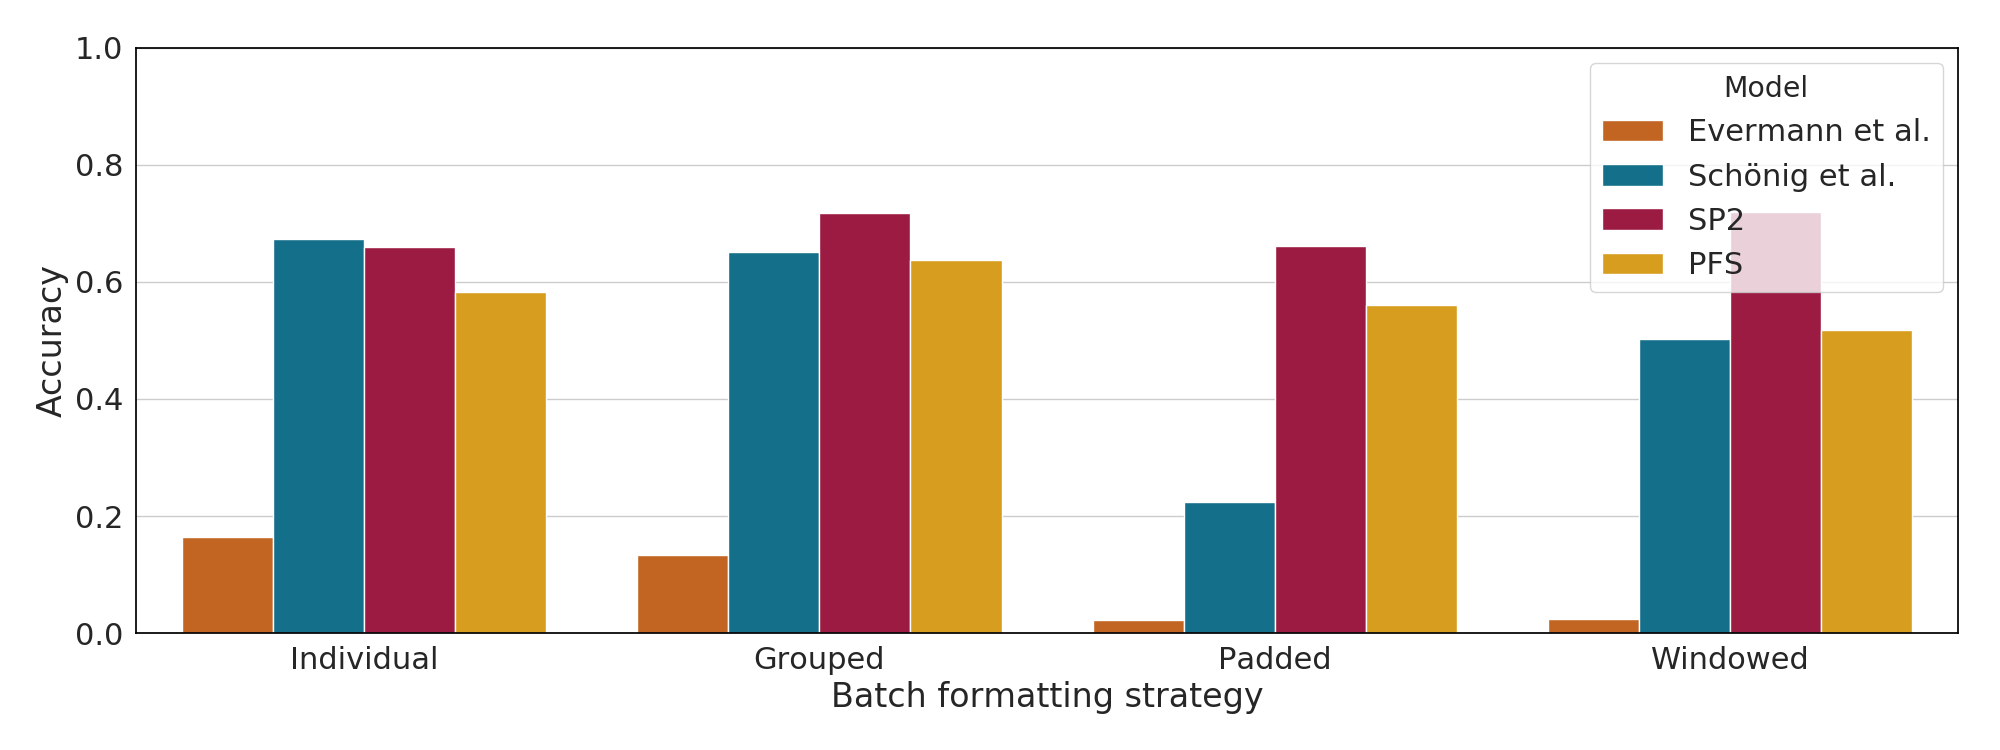
\includegraphics[width=\textwidth]{gfx/bpic2015_4/accuracies.png}
    \caption{Best accuracies obtained on the validation set on the BPI15-4 data}
    \label{fig:max-accuracies-bpic2015-4}
\end{figure}
\begin{figure}
    \centering
    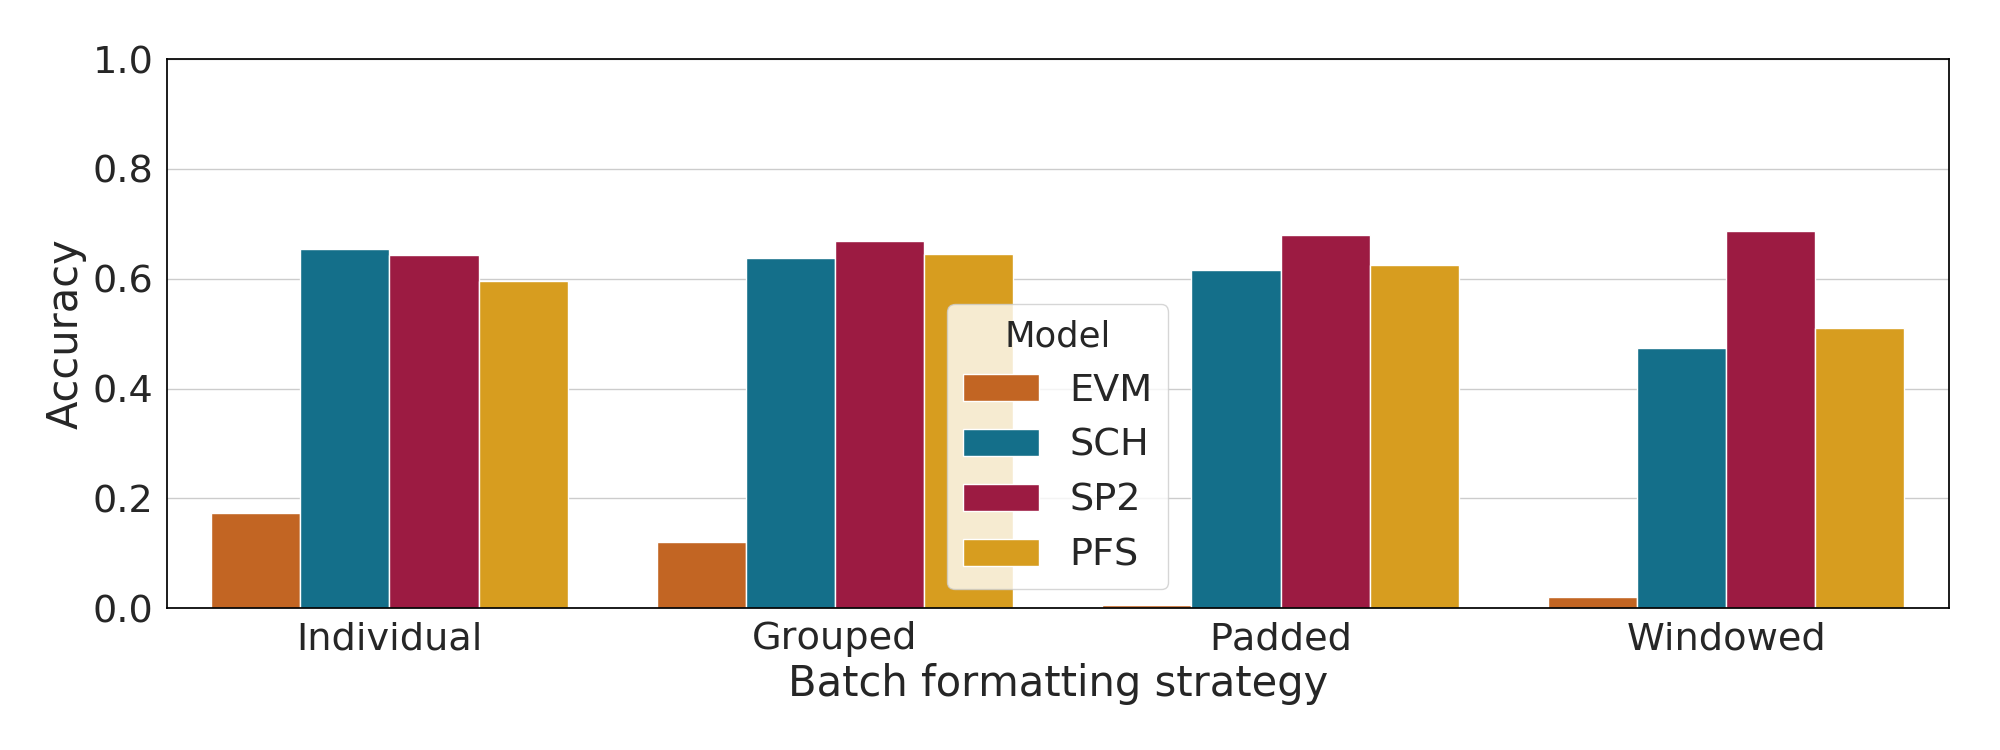
\includegraphics[width=\textwidth]{gfx/bpic2015_5/accuracies.png}
    \caption{Best accuracies obtained on the validation set on the BPI15-5 data}
    \label{fig:max-accuracies-bpic2015-5}
\end{figure}

\FloatBarrier
\subsection*{Training times}
The batch size is an important hyper-parameter, and since it directly corresponds to the number of weight adjustments per epoch, it also impacts the time that the training of an epoch requires. 
\begin{figure}[!htb]
    \centering
    \subfloat[][Training times measured on the BPIC11~\cite{BPIC2011} dataset]{
        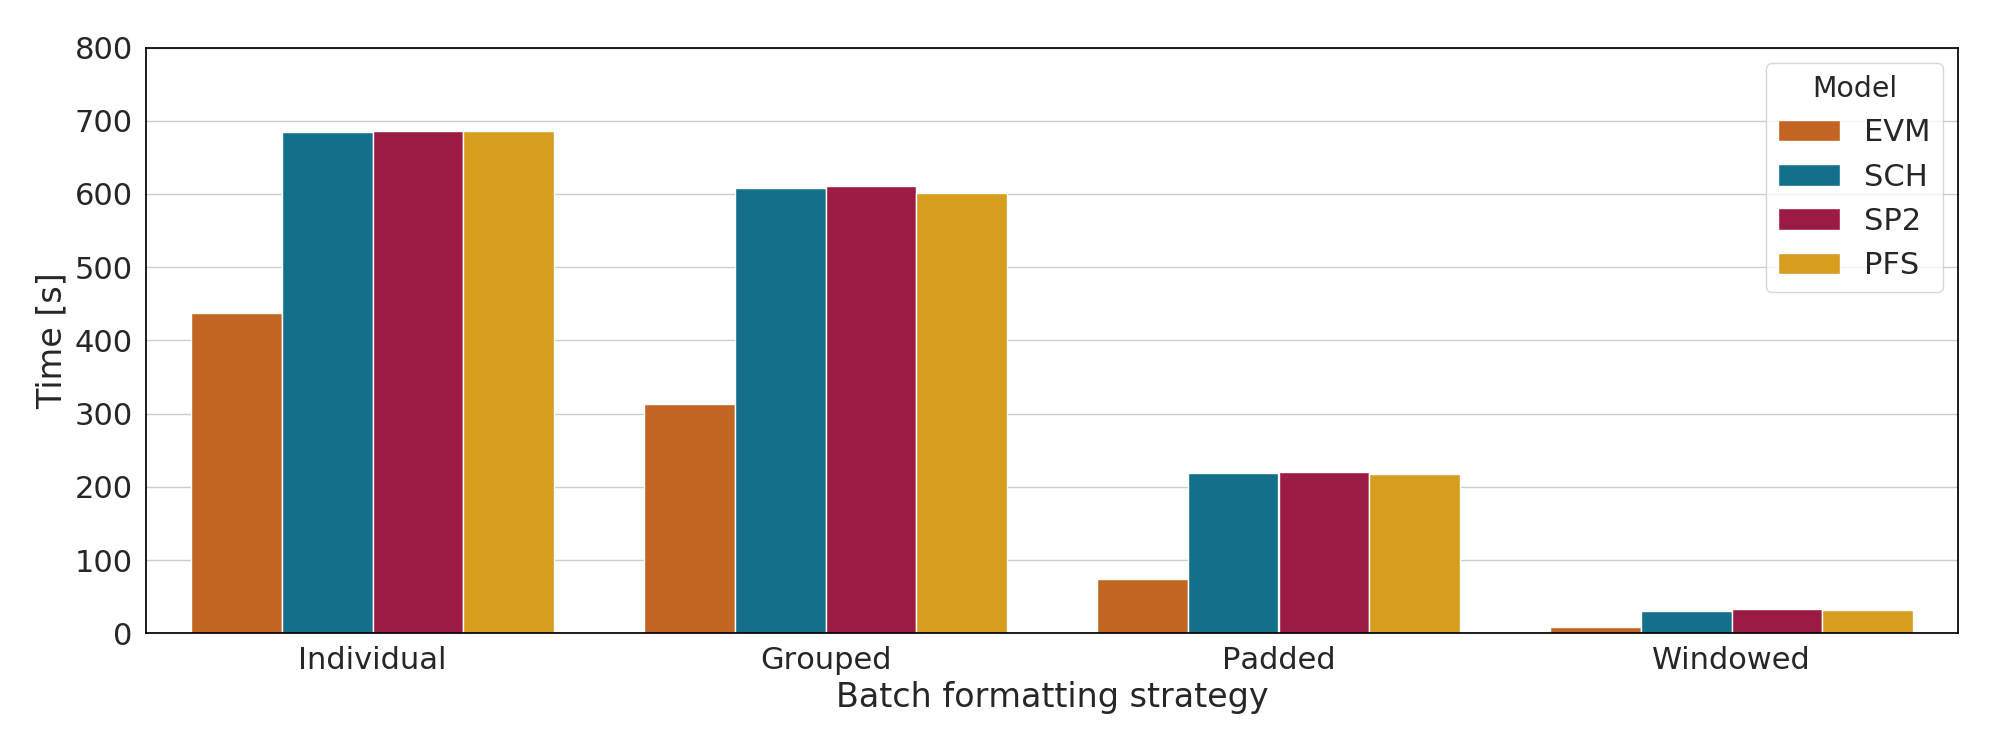
\includegraphics[width=\textwidth]{gfx/bpic2011/train_timings.png}
        \label{fig:BPIC11-training-timings}
    }
    \qquad
    \subfloat[][Training times measured on the BPIC12~\cite{BPIC2012} dataset]{
        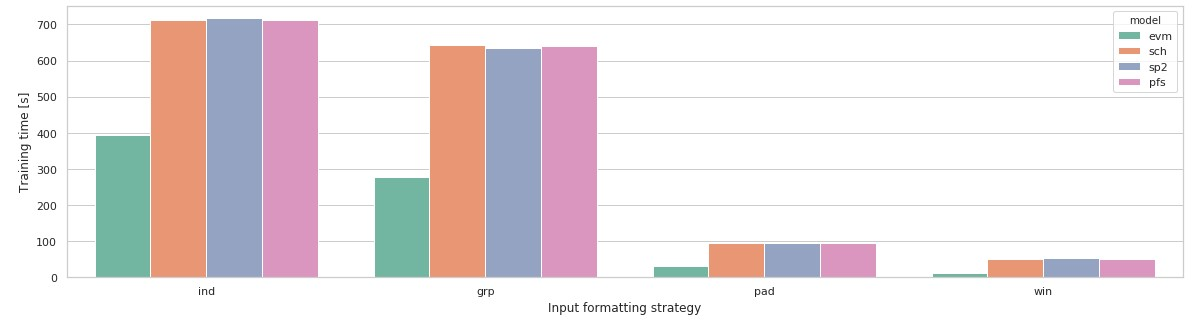
\includegraphics[width=\textwidth]{gfx/bpic11-training-timings.jpg}
        \label{fig:BPIC12-training-timings}
    }
    \qquad
    \subfloat[][Training times measured on the BPIC17~\cite{BPIC2017} dataset]{
        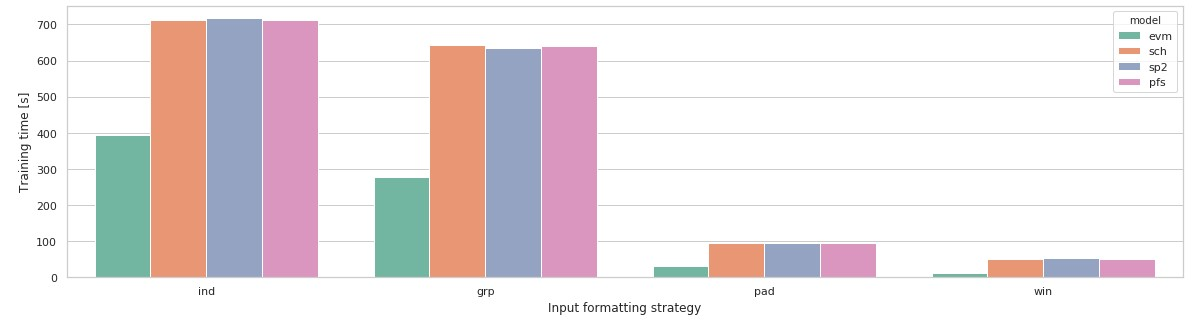
\includegraphics[width=\textwidth]{gfx/bpic11-training-timings.jpg}
        \label{fig:BPIC17-training-timings}
    }
    
    \caption{Training times per epoch for each model-formatting combination, listed per dataset}
    \label{fig:training-timings}
\end{figure}

\FloatBarrier
\subsection*{Stability}
wasd

\section{Discussion}\label{sec:eval:discussion}
\todo[inline]{Is this really needed? Maybe discuss directly with the results?}